\chapter{Routing}

Even nowadays the routing is often done manually for analogue circuits. This is mainly caused by a lack of good tools and therefore the missing trust of engineers in them. The engineers consider a lot of different constraints during the routing, for example symmetries, net lengths and capacitive couplings. All these things have a major impact on the performance of the circuit, as in the analogue world it is very important to have a really accurate signal level, only high or low isn't enough.

The designer additonally adds guards and rings to the placement to protect certain devices from noise. This noise can come from for example the clock net or other routes, which carry a signal with high frequency. But high frequencies aren't the only disturbing effects, already during the placement the designer has to consider temperature gradients, caused by transistors with a high power consumption. To avoid problems with different temperatures in the substrate of for example the devices of differential pair the can be placed symmetric or can even have a common centroid. Around these grouped modules then the designer can create for example a guard ring around to protect the devices even more. An example for a manually routed layout can be seen in [\ref{fig:miller_amplifier_routed_layout}].

So for an automatic routing algorithm a lot of different constraints have to considered. There are even more obstacles than just the devices and already created routes, for example the routes should pass over guard rings. To solve this problem in the following chapter are two different approaches presented: One simple sequentially line expansion router and one extend version of the previous one, which selects all routes together in one step. But first I have to discuss the changes that were necessary for the implementation of the routing algorithms.

%\begin{figure}
%	\centering
%	\includegraphics[scale=.3]{FIG/miller_amplifier_routed_layout.png}
%  	\caption{routed layout of a miller amplifier}
%	\label{fig:miller_amplifier_routed_layout}
%\end{figure}
PICTURE MISSING MILLER AMPLIFIER ROUTED LAYOUT

\section{Changes for Routing in the existing Applications}

\subsection{Plantage}

\subsubsection{Missing Data}
To actually route the placements some data was missing in plantage. Although at some points the routing was already prepared, example given the net names were available, but important information was not given. These include:
\begin{itemize}
\item Actual dimensions of the modules
\item Parameters for the technology
\item Vias and routes
\item Guard rings
\end{itemize}

In awareness of the necessary routing for every module a bigger area was defined for the placement. The additional space between the modules could then be used to route the placement. But the information about the actual dimension of the modules was missing.

The technology rules are passed through by the ICFBInterface to Plantage. At least for the technology definitions of Austria Microsystems it is not necessary to convert these rules, as the same format is chosen. For other manufacturers a conversion might be necessary.

The vias and routes were not considered at all previously. The main information which is needed to route are the dimension of the vias on the different layers and the width for the routes. Actually there is no real width for a route, but a minimal width, which a route must have. Usually this width is used for the routes. Also the dimensions for the via must be caculated, which can be done as described previously. Also the generated routes and placed vias needed to be added to the output of plantage, so that they can be shown in the GUI.

Previously every pin consisted only of one rectangle, which is obviously not enough. This basic information was used to minimize the estimated net length for the placements. But for real routing we need more complex possibilities to define pins, as, for example, the gate can be connected from both sides. Also it is not recommend to contact over the diffusion area. This will result in even more complex contact areas, as they could be split up in different parts. The definition of these areas is done by the user in the GUI and handed over to plantage. The used format defines for every pin, which a module has, at least one contact area, but eventually a lot more. During the routing then the acutal contact area is selected based on a certain heuristic.

\subsubsection{Treatment of Groups}

\subsection{ICFBInterface}
The GUI-part of this application also needed some adaptions. This work was mainly done by Martin Keßler and contained the following parts:

\begin{itemize}
\item possibility to define contact areas
\item displaying routes and vias
\item possibility to change algorithm settings
\end{itemize}	

\section{Overview of Existing Routing Algorithms}

\section{Implemented Routing Algorithms}
During this thesis two different routing algorithms were implemented: First of all a typical line expansion router. This solutions doesn't consider all constraints, but it is able to create at least reasonable results. Afterwards this algorithm was extended to consider additional constraints.

\subsection{Line Expansion Router}
The first thing which the algorithm has to do, before it can calculate a route, is to selected the start and target contact area. There can be several possibilities, as every pin can have several contact areas. Later on we will even see that already created routes can be candidates to start or end with a route. Basically this task can be seen as the selection of the closest rectangles of two lists of possibilities. For this I first want to talk a little bit about how the closest distance between two rectangles can be calculated.

For two rectangles there are several possible constellations. The first one we usually check is, if the overlap. If this is the case we can calculated easily the rectangle which is covered by both [\ref{fig:rectangles_overlapping}]. The distance is 0 in this case, and as start points for both rectangles we can select the center of gravity of the overlapping area.

\begin{figure}
	\centering
	\setlength{\unitlength}{0.282222229121mm}
\begin{picture}(275.80054, 174.07812)(0, -174.07812)
  \put(0,-174.07812){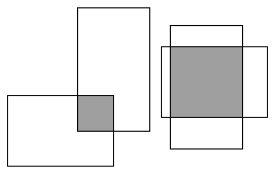
\includegraphics[height=49.1287150676mm, width=77.8370431916mm]{FIG/rectangles_overlapping.svg.pdf}}
\end{picture}
  	\caption{overlapping area of two rectangles is again a rectangle}
	\label{fig:rectangles_overlapping}
\end{figure}

If the two rectangles do not overlap it becomes a little bit more difficult. In this case we can at least say, that one of the rectangle has its closest point at one of the. Actually there can be even an endless count of solutions for this problem, but we are only interested in one of them. Because of this we select the easiest to calculate solution, which means the selection of a corner for one rectangle. The closest corner from the first rectangle to the second one is that one, which has the closest euclidean distance to the center of gravity of the second one [\ref{fig:rectangles_closest_corner}]. As we now know for one rectangle the closest point we can start to select the closest point on the second one. This point must be obviously on one of the edges. Every edges is basically a line segment, where the closest point can be calculated easily. For this task we first need the expansion of the line segment into a whole line. We then can turn this line 90 degrees (it doesn't matter in which direction as it is a line) and move this new line, so that it crosses our point, from which we want to know the closest point on the line segment. The crossing point of these two lines, if it is also inside the line segment, is the closest point. If this crossing point is outside the line segment the closest point must be the start or end point of the line segment, which are actually the rectangle's corners.

\begin{figure}
	\centering
	\setlength{\unitlength}{0.282222229121mm}
\begin{picture}(275.80054, 174.07812)(0, -174.07812)
  \put(0,-174.07812){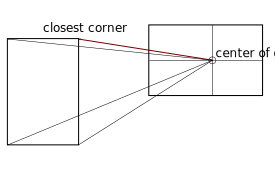
\includegraphics[height=49.1287150676mm, width=77.8370431916mm]{FIG/rectangles_closest_corner.svg.pdf}}
  \put(216.142843,-57.22096){\makebox(0,0)[l]{\smash{center of gravity}}}
  \put(43.019685,-31.84584){\makebox(0,0)[l]{\smash{closest corner}}}
\end{picture}
  	\caption{the closest corner is that one, which has the smallest distance to the center of gravity of the other one}
	\label{fig:rectangles_closest_corner}
\end{figure}

After the algorithm has selected start and target contact areas the next step is to avoid routes across modules. For this purpose during all the following steps the modules are considered as obstacles. But during the first step usually the route has first to get out of the module. To avoid additional, accidentally added, gates the algorithm has to choose the shortest way to get out of the module. To decrease the resistance it is also possible to start right at the contact area to the next layer and use for example metal to get out of the module as fast as possible.

As the algorithm now has all the necessary information the actual line expansion routing can start. The main idea behind a line expansion router is that the routes are created sequentially. Every single step is based on a map of obstacles, which the route mustn't cross. From the starting point beginning always the next possible point of a route is calculated and the algorithm afterwards again applied to this partial problem. At the beginning of this recursive algorithm, as usual, the terminating condition is checked: If we have reached the target point. In every single step there are several decisions to be made: First the possible directions are grouped in good and bad directions [\ref{fig:good_and_bad_directions}]. Good directions are those, which reduce the distance to the target and bad ones are all the others.

%\begin{figure}
%	\centering
%	\input{FIG/good_and_bad_directions.svg}
%  	\caption{good and bad directions}
%	\label{fig:good_and_bad_directions}
%\end{figure}
PICTURE MISSING GOOD AND BAD DIRECTIONS

Additionally it makes no sense to go back the same direction where the last step came from. Also the same direction like the last step is not senseful. Because if this would be a good decision, the last step could have gone further. So these two directions are removed from the good directions. After this selection the router can make one step further in every good directon, as far as possible. This means, that the next step can go as far, as no obstacle is on the way or the target (in this coordinate) is reached [\ref{fig:router_go_as_far_as_possible}].

%\begin{figure}
%	\centering
%	\input{FIG/router_go_as_far_as_possible.svg}
%  	\caption{one step into a good direction can go as far as possible}
%	\label{fig:router_go_as_far_as_possible}
%\end{figure}
PICTURE MISSING ROUTER GO AS FAR AS POSSIBLE

During the calculation of the steps towards the target we count those, which are feasible. If none of them is feasible the algorithm will have to select one of the bad directions for the next step. A major premission for this is also, that our last step ended at an obstacle. The router now can go as far as necessary into this bad direction [\ref{fig:router_go_as_far_as_necessary}].

%\begin{figure}
%	\centering
%	\input{FIG/router_go_as_far_as_necessary.svg}
% 	\caption{one step into a bad direction should go only as far as necessary}
%	\label{fig:router_go_as_far_as_necessary}
%\end{figure}
PICTURE MISSING ROUTER GO AS FAR AS NECESSARY

Last but no least it is also possible to switch to the neighboured layers.

Finally, if the start point is the same as the end point the algorithm has calculated a feasible and complete route. This result is added to all the possible routes for this necessary connection. From these possible routes the first, quite simple, algorithm chooses only the best one. As this algorithm calculates the routes sequentially it has no information about for example symmetries or other parasitics, therefore the \textit{best} possibility is chosen on the lowest resistance.

Typically there are several pins on every net, which means the algorithm has to calculate no only one route per net. To reduce the net length all the already calculated and selected routes are added as possible targets for the next routes.

For this first algorithm a lot of different possibilities for every necessary connection is quite a lot of information, as it chooses only the shortest one in terms of resistance. But the results, which we generate here, can be reused for the next, extended, version of the line expansion algorithm.

\subsection{Extended Line Expansion Router}